% NLP1 Project 1, group 24: five backup slides for the oral assessment (SST-2 sentiment classification).
% Build: tectonic slides.tex   (or pdflatex slides.tex)
\documentclass[aspectratio=169,10pt]{beamer}

\usepackage[T1]{fontenc}
\usepackage{lmodern}
\usepackage{amssymb}
\usepackage{tikz}
\usetikzlibrary{arrows.meta,positioning,calc,plotmarks}

% ---------- palette ----------
\definecolor{ink}{HTML}{1F2937}
\definecolor{muted}{HTML}{6B7280}
\definecolor{accent}{HTML}{1D4ED8}
\definecolor{neg}{HTML}{C2410C}
\definecolor{pos}{HTML}{0F766E}
\definecolor{amber}{HTML}{B7791F}
\definecolor{panel}{HTML}{F3F4F6}
\definecolor{rule}{HTML}{D1D5DB}

% ---------- theme ----------
\usetheme{default}
\renewcommand{\familydefault}{\sfdefault}
\setbeamertemplate{navigation symbols}{}
\setbeamercolor{normal text}{fg=ink}
\setbeamercolor{structure}{fg=accent}
\setbeamersize{text margin left=9mm,text margin right=9mm}
\setlength{\parskip}{0pt}

\setbeamertemplate{frametitle}{%
  \nointerlineskip\vskip2.6mm
  {\Large\bfseries\color{ink}\insertframetitle}\par\vskip0.4mm
  {\color{accent}\rule{\textwidth}{0.7pt}}\vskip0.8mm}
\setbeamertemplate{footline}{%
  \hbox to\paperwidth{\hspace{9mm}{\color{muted}\tiny NLP1 \,$\cdot$\, Project 1 \,$\cdot$\, Group 24 \,$\cdot$\, SST-2 sentiment}%
  \hfill{\color{muted}\tiny backup slide \insertframenumber/\inserttotalframenumber}\hspace{9mm}}\vskip2.6mm}

\tikzset{
  every picture/.style={font=\scriptsize,>={Stealth[length=1.6mm]}},
  neuron/.style={circle,draw=ink!55,fill=white,minimum size=2.3mm,inner sep=0},
  ttl/.style={anchor=south west,inner sep=0,font=\footnotesize\bfseries},
  note/.style={inner sep=1pt,font=\tiny,text=muted},
}
\newcommand{\lab}[1]{\textcolor{muted}{#1}}
\newcommand{\num}[1]{\textcolor{accent}{#1}\;}   % panel number
% accuracy -> cm for the plots (defined here: macros with # cannot be defined inside a frame)
\newcommand{\xr}[1]{((#1-0.780)*150)}  % slide 2, representation plot
\newcommand{\ya}[1]{((#1-0.780)*85)}   % slide 3, activation plot
\newcommand{\xa}[1]{((#1-0.770)*62)}   % slide 4, accuracy plot

\begin{document}

% =====================================================================
% 1  DATA AND METRICS
% =====================================================================
\begin{frame}{1 \,$\cdot$\, Data and metrics}
\begin{columns}[T]
% ---- 1. train is mostly short sub-phrases ----
\begin{column}{0.47\textwidth}
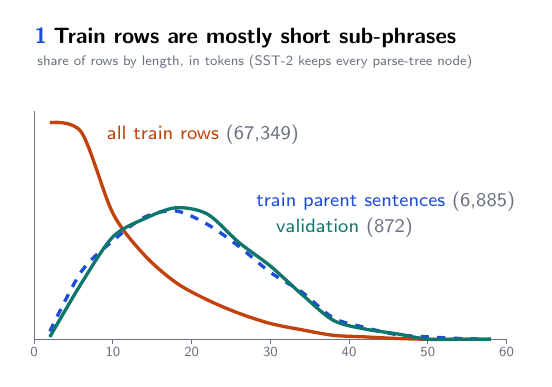
\begin{tikzpicture}[x=1cm,y=1cm]
  \node[ttl] at (0,0.3) {\num{1}Train rows are mostly short sub-phrases};
  \node[note,anchor=west] at (0,0.12) {share of rows by length, in tokens (SST-2 keeps every parse-tree node)};
  \def\b{-3.4}
  \draw[muted] (0,\b) -- (6.0,\b); \draw[muted] (0,\b) -- (0,{\b+2.9});
  \foreach \t in {0,10,20,30,40,50,60}{\draw[muted] (\t*0.1,\b) -- ++(0,-0.06); \node[note,below] at (\t*0.1,{\b-0.06}) {\t};}
  \draw[neg,very thick] plot[smooth] coordinates {(0.2,{\b+2.75}) (0.6,{\b+2.63}) (1.0,{\b+1.60}) (1.4,{\b+1.07}) (1.8,{\b+0.72}) (2.2,{\b+0.50}) (2.6,{\b+0.33}) (3.0,{\b+0.20}) (3.4,{\b+0.12}) (3.8,{\b+0.05}) (4.2,{\b+0.03}) (4.6,{\b+0.01}) (5.0,\b) (5.4,\b) (5.8,\b)};
  \draw[accent,very thick,dashed] plot[smooth] coordinates {(0.2,{\b+0.10}) (0.6,{\b+0.86}) (1.0,{\b+1.25}) (1.4,{\b+1.55}) (1.8,{\b+1.63}) (2.2,{\b+1.46}) (2.6,{\b+1.18}) (3.0,{\b+0.85}) (3.4,{\b+0.60}) (3.8,{\b+0.27}) (4.2,{\b+0.15}) (4.6,{\b+0.06}) (5.0,{\b+0.03}) (5.4,{\b+0.01}) (5.8,\b)};
  \draw[color=pos,very thick] plot[smooth] coordinates {(0.2,{\b+0.03}) (0.6,{\b+0.71}) (1.0,{\b+1.30}) (1.4,{\b+1.53}) (1.8,{\b+1.67}) (2.2,{\b+1.59}) (2.6,{\b+1.23}) (3.0,{\b+0.93}) (3.4,{\b+0.57}) (3.8,{\b+0.24}) (4.2,{\b+0.13}) (4.6,{\b+0.07}) (5.0,\b) (5.4,\b) (5.8,\b)};
  \node[anchor=west,text=neg] at (0.8,{\b+2.6}) {all train rows \lab{(67,349)}};
  \node[anchor=west,text=accent] at (2.7,{\b+1.75}) {train parent sentences \lab{(6,885)}};
  \node[anchor=west,text=pos] at (2.95,{\b+1.42}) {validation \lab{(872)}};
\end{tikzpicture}
\end{column}

% ---- 2. random folds leak ----
\begin{column}{0.47\textwidth}
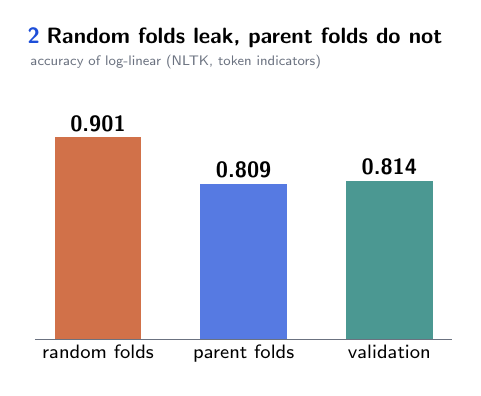
\begin{tikzpicture}[x=1cm,y=1cm]
  \node[ttl] at (0,0.3) {\num{2}Random folds leak, parent folds do not};
  \node[note,anchor=west] at (0,0.12) {accuracy of log-linear (NLTK, token indicators)};
  \def\b{-3.4}
  \def\s{6.4}   % cm per accuracy unit above 0.5
  \foreach \x/\v/\c/\t in {0.9/0.901/neg/random folds, 2.75/0.809/accent/parent folds, 4.6/0.814/pos/validation}{
    \fill[\c!75] (\x-0.55,\b) rectangle (\x+0.55,{\b+(\v-0.5)*\s});
    \node[above,inner sep=2pt,font=\footnotesize\bfseries] at (\x,{\b+(\v-0.5)*\s}) {\v};
    \node[below,inner sep=2pt] at (\x,\b) {\t};}
  \draw[muted] (0.1,\b) -- (5.4,\b);
\end{tikzpicture}
\end{column}
\end{columns}
\end{frame}

% =====================================================================
% 2  FEATURES
% =====================================================================
\begin{frame}{2 \,$\cdot$\, Features}
\begin{columns}[T]
% ---- 1. tokenisers ----
\begin{column}{0.47\textwidth}
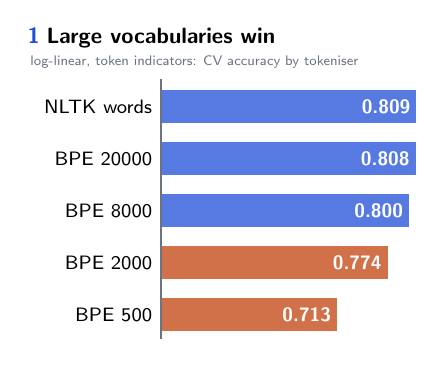
\begin{tikzpicture}[x=1cm,y=1cm]
  \node[ttl] at (-1.7,0.3) {\num{1}Large vocabularies win};
  \node[note,anchor=west] at (-1.7,0.12) {log-linear, token indicators: CV accuracy by tokeniser};
  \def\s{10.5}  % cm per accuracy unit above 0.5
  \foreach \i/\v/\t/\c in {0/0.809/NLTK words/accent, 1/0.808/BPE 20000/accent, 2/0.800/BPE 8000/accent, 3/0.774/BPE 2000/neg, 4/0.713/BPE 500/neg}{
    \pgfmathsetmacro{\y}{-0.45-\i*0.66}
    \fill[\c!75] (0,{\y+0.21}) rectangle ({(\v-0.5)*\s},{\y-0.21});
    \node[anchor=east,inner sep=3pt] at (0,\y) {\t};
    \node[anchor=east,inner sep=2pt,font=\scriptsize\bfseries,text=white] at ({(\v-0.5)*\s},\y) {\v};}
  \draw[muted] (0,-0.1) -- (0,-3.4);
\end{tikzpicture}
\end{column}

% ---- 2. representations ----
\begin{column}{0.47\textwidth}
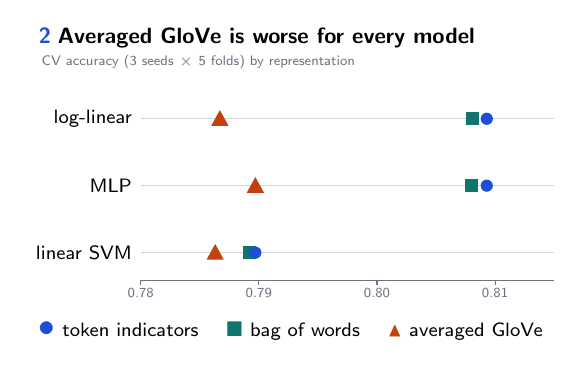
\begin{tikzpicture}[x=1cm,y=1cm]
  \node[ttl] at (-1.3,0.3) {\num{2}Averaged GloVe is worse for every model};
  \node[note,anchor=west] at (-1.3,0.12) {CV accuracy (3 seeds $\times$ 5 folds) by representation};
  \foreach \i/\n/\a/\b/\g in {0/log-linear/0.8093/0.8081/0.7867, 1/MLP/0.8093/0.8080/0.7897, 2/linear SVM/0.7897/0.7892/0.7863}{
    \pgfmathsetmacro{\y}{-0.6-\i*0.85}
    \node[anchor=east,inner sep=3pt] at (0,\y) {\n};
    \draw[rule] (0,\y) -- ({\xr{0.815}},\y);
    \fill[neg] ({\xr{\g}},\y) ++(0,0.11) -- ++(0.11,-0.2) -- ++(-0.22,0) -- cycle;
    \fill[color=pos] ({\xr{\b}-0.08},\y-0.08) rectangle ++(0.16,0.16);
    \fill[accent] ({\xr{\a}},\y) circle (2.2pt);}
  \draw[muted] (0,-2.65) -- ({\xr{0.815}},-2.65);
  \foreach \a in {0.78,0.79,0.80,0.81}{\draw[muted] ({\xr{\a}},-2.65) -- ++(0,-0.06); \node[note,below] at ({\xr{\a}},-2.71) {\a};}
  \node[anchor=west,inner sep=0] at (-1.3,-3.3) {\textcolor{accent}{\large$\bullet$} token indicators \quad \textcolor{pos}{$\blacksquare$} bag of words \quad \textcolor{neg}{$\blacktriangle$} averaged GloVe};
\end{tikzpicture}
\end{column}
\end{columns}
\end{frame}

% =====================================================================
% 3  ARCHITECTURES
% =====================================================================
\begin{frame}{3 \,$\cdot$\, Architectures}
\begin{columns}[T]
% ---- 1. the four architectures ----
\begin{column}{0.47\textwidth}
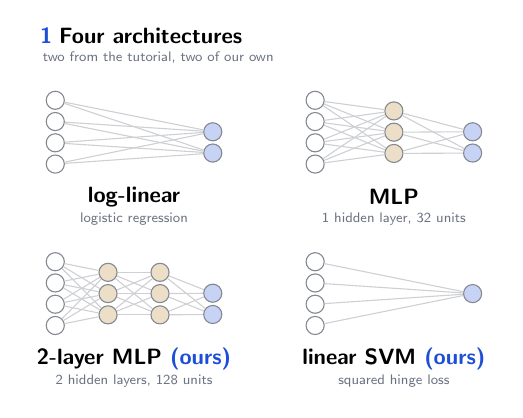
\begin{tikzpicture}[x=1cm,y=1cm]
  \node[ttl] at (0,0.3) {\num{1}Four architectures};
  \node[note,anchor=west] at (0,0.12) {two from the tutorial, two of our own};
  % log-linear
  \begin{scope}[shift={(0.2,-0.15)}]
    \foreach \i in {1,...,4}{\node[neuron] (a\i) at (0,-\i*0.27) {};}
    \foreach \i in {1,2}{\node[neuron,fill=accent!25] (o\i) at (2.0,-0.4-\i*0.27) {};}
    \foreach \i in {1,...,4}{\foreach \j in {1,2}{\draw[ink!22] (a\i)--(o\j);}}
    \node[font=\footnotesize\bfseries] at (1.0,-1.5) {log-linear};
    \node[note] at (1.0,-1.78) {logistic regression};
  \end{scope}
  % MLP
  \begin{scope}[shift={(3.5,-0.15)}]
    \foreach \i in {1,...,4}{\node[neuron] (a\i) at (0,-\i*0.27) {};}
    \foreach \i in {1,...,3}{\node[neuron,fill=amber!25] (h\i) at (1.0,-0.135-\i*0.27) {};}
    \foreach \i in {1,2}{\node[neuron,fill=accent!25] (o\i) at (2.0,-0.4-\i*0.27) {};}
    \foreach \i in {1,...,4}{\foreach \j in {1,...,3}{\draw[ink!22] (a\i)--(h\j);}}
    \foreach \i in {1,...,3}{\foreach \j in {1,2}{\draw[ink!22] (h\i)--(o\j);}}
    \node[font=\footnotesize\bfseries] at (1.0,-1.5) {MLP};
    \node[note] at (1.0,-1.78) {1 hidden layer, 32 units};
  \end{scope}
  % 2-layer MLP
  \begin{scope}[shift={(0.2,-2.2)}]
    \foreach \i in {1,...,4}{\node[neuron] (a\i) at (0,-\i*0.27) {};}
    \foreach \i in {1,...,3}{\node[neuron,fill=amber!25] (h\i) at (0.67,-0.135-\i*0.27) {};}
    \foreach \i in {1,...,3}{\node[neuron,fill=amber!25] (g\i) at (1.33,-0.135-\i*0.27) {};}
    \foreach \i in {1,2}{\node[neuron,fill=accent!25] (o\i) at (2.0,-0.4-\i*0.27) {};}
    \foreach \i in {1,...,4}{\foreach \j in {1,...,3}{\draw[ink!22] (a\i)--(h\j);}}
    \foreach \i in {1,...,3}{\foreach \j in {1,...,3}{\draw[ink!22] (h\i)--(g\j);}}
    \foreach \i in {1,...,3}{\foreach \j in {1,2}{\draw[ink!22] (g\i)--(o\j);}}
    \node[font=\footnotesize\bfseries] at (1.0,-1.5) {2-layer MLP \textcolor{accent}{(ours)}};
    \node[note] at (1.0,-1.78) {2 hidden layers, 128 units};
  \end{scope}
  % linear SVM
  \begin{scope}[shift={(3.5,-2.2)}]
    \foreach \i in {1,...,4}{\node[neuron] (a\i) at (0,-\i*0.27) {};}
    \node[neuron,fill=accent!25] (o) at (2.0,-0.675) {};
    \foreach \i in {1,...,4}{\draw[ink!22] (a\i)--(o);}
    \node[font=\footnotesize\bfseries] at (1.0,-1.5) {linear SVM \textcolor{accent}{(ours)}};
    \node[note] at (1.0,-1.78) {squared hinge loss};
  \end{scope}
\end{tikzpicture}
\end{column}

% ---- 2. the non-linearity barely matters ----
\begin{column}{0.47\textwidth}
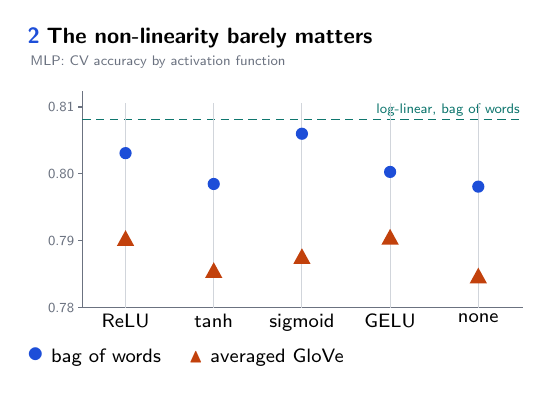
\begin{tikzpicture}[x=1cm,y=1cm]
  \node[ttl] at (-0.7,0.3) {\num{2}The non-linearity barely matters};
  \node[note,anchor=west] at (-0.7,0.12) {MLP: CV accuracy by activation function};
  \def\b{-3.0}
  \draw[muted] (0,\b) -- (5.6,\b); \draw[muted] (0,\b) -- (0,{\b+2.75});
  \foreach \a in {0.78,0.79,0.80,0.81}{\draw[muted] (0,{\b+\ya{\a}}) -- ++(-0.06,0); \node[note,left] at (-0.06,{\b+\ya{\a}}) {\a};}
  \draw[color=pos,densely dashed] (0,{\b+\ya{0.8081}}) -- (5.6,{\b+\ya{0.8081}});
  \node[note,text=pos,anchor=south east] at (5.6,{\b+\ya{0.8081}}) {log-linear, bag of words};
  \foreach \i/\n/\bw/\g in {0/ReLU/0.8031/0.7903, 1/tanh/0.7985/0.7855, 2/sigmoid/0.8060/0.7876, 3/GELU/0.8003/0.7905, 4/none/0.7981/0.7847}{
    \pgfmathsetmacro{\x}{0.55+\i*1.12}
    \draw[rule] (\x,\b) -- (\x,{\b+2.6});
    \fill[accent] (\x,{\b+\ya{\bw}}) circle (2.2pt);
    \fill[neg] (\x,{\b+\ya{\g}}) ++(0,0.11) -- ++(0.11,-0.2) -- ++(-0.22,0) -- cycle;
    \node[below,inner sep=2pt] at (\x,\b) {\n};}
  \node[anchor=west,inner sep=0] at (-0.7,{\b-0.62}) {\textcolor{accent}{\large$\bullet$} bag of words \quad \textcolor{neg}{$\blacktriangle$} averaged GloVe};
\end{tikzpicture}
\end{column}
\end{columns}
\end{frame}

% =====================================================================
% 4  RESULTS
% =====================================================================
\begin{frame}{4 \,$\cdot$\, Results}
\begin{center}
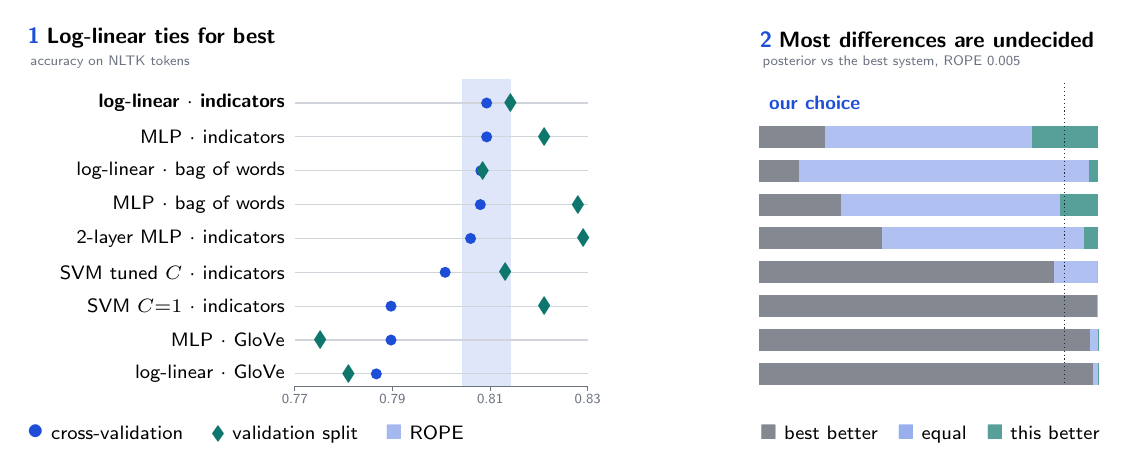
\begin{tikzpicture}[x=1cm,y=1cm]
  \def\bx{5.9}   % start of the probability bars
  \def\bw{4.3}   % their width
  \node[ttl] at (-3.4,0.55) {\num{1}Log-linear ties for best};
  \node[note,anchor=west] at (-3.4,0.37) {accuracy on NLTK tokens};
  \node[ttl] at (\bx,0.55) {\num{2}Most differences are undecided};
  \node[note,anchor=west] at (\bx,0.37) {posterior vs the best system, ROPE 0.005};
  % ROPE band around the best system
  \fill[accent!14] ({\xa{0.8043}},0.15) rectangle ({\xa{0.8143}},-3.75);
  \foreach \i/\t/\cv/\va/\pb/\pt in {
     0/log-linear $\cdot$ indicators/0.8093/0.8142/0/0,
     1/MLP $\cdot$ indicators/0.8093/0.8211/0.195/0.610,
     2/log-linear $\cdot$ bag of words/0.8081/0.8085/0.116/0.857,
     3/MLP $\cdot$ bag of words/0.8080/0.8280/0.240/0.647,
     4/2-layer MLP $\cdot$ indicators/0.8060/0.8291/0.362/0.597,
     5/SVM tuned $C$ $\cdot$ indicators/0.8008/0.8131/0.870/0.130,
     6/SVM $C{=}1$ $\cdot$ indicators/0.7897/0.8211/0.998/0.002,
     7/MLP $\cdot$ GloVe/0.7897/0.7752/0.975/0.024,
     8/log-linear $\cdot$ GloVe/0.7867/0.7810/0.986/0.013}{
    \pgfmathsetmacro{\y}{-0.15-\i*0.43}
    \ifnum\i=0
      \node[anchor=east,inner sep=2pt,font=\scriptsize\bfseries] at (-0.05,\y) {\t};
      \node[anchor=west,font=\scriptsize\bfseries,text=accent] at (\bx,\y) {our choice};
    \else
      \node[anchor=east,inner sep=2pt] at (-0.05,\y) {\t};
      \fill[ink!55]    (\bx,{\y+0.14}) rectangle ({\bx+\pb*\bw},{\y-0.14});
      \fill[accent!35] ({\bx+\pb*\bw},{\y+0.14}) rectangle ({\bx+(\pb+\pt)*\bw},{\y-0.14});
      \fill[pos!70]    ({\bx+(\pb+\pt)*\bw},{\y+0.14}) rectangle ({\bx+\bw},{\y-0.14});
    \fi
    \draw[rule] (0,\y) -- ({\xa{0.830}},\y);
    \fill[accent] ({\xa{\cv}},\y) circle (2pt);
    \node[text=pos,inner sep=0,font=\footnotesize] at ({\xa{\va}},\y) {$\blacklozenge$};}
  \draw[ink,densely dotted] ({\bx+0.9*\bw},0.1) -- ({\bx+0.9*\bw},-3.7);
  % accuracy axis
  \draw[muted] (0,-3.75) -- ({\xa{0.830}},-3.75);
  \foreach \a in {0.77,0.79,0.81,0.83}{\draw[muted] ({\xa{\a}},-3.75) -- ++(0,-0.06); \node[note,below] at ({\xa{\a}},-3.81) {\a};}
  \node[anchor=west,inner sep=0] at (-3.4,-4.35) {\textcolor{accent}{\large$\bullet$} cross-validation \quad \textcolor{pos}{$\blacklozenge$} validation split \quad \textcolor{accent!40}{$\blacksquare$} ROPE};
  \node[anchor=west,inner sep=0] at (\bx,-4.35) {\textcolor{ink!55}{$\blacksquare$} best better \; \textcolor{accent!45}{$\blacksquare$} equal \; \textcolor{pos!70}{$\blacksquare$} this better};
\end{tikzpicture}
\end{center}
\end{frame}

% =====================================================================
% 5  EXTRA: why every model stops at about 81%
% =====================================================================
\begin{frame}{5 \,$\cdot$\, Extra: why every model stops at about 81\%}
\begin{columns}[T]
% ---- 1. hard sentence types ----
\begin{column}{0.47\textwidth}
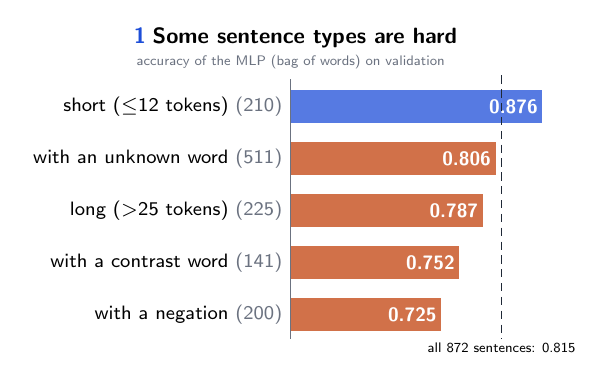
\begin{tikzpicture}[x=1cm,y=1cm]
  \node[ttl] at (-2.0,0.3) {\num{1}Some sentence types are hard};
  \node[note,anchor=west] at (-2.0,0.12) {accuracy of the MLP (bag of words) on validation};
  \def\s{8.5}   % cm per accuracy unit above 0.5
  \def\all{0.815}
  \foreach \i/\t/\n/\v/\col in {
     0/short ($\leq$12 tokens)/210/0.876/accent,
     1/with an unknown word/511/0.806/neg,
     2/long ($>$25 tokens)/225/0.787/neg,
     3/with a contrast word/141/0.752/neg,
     4/with a negation/200/0.725/neg}{
    \pgfmathsetmacro{\y}{-0.45-\i*0.66}
    \fill[\col!75] (0,{\y+0.21}) rectangle ({(\v-0.5)*\s},{\y-0.21});
    \node[anchor=east,inner sep=2pt,font=\scriptsize] at (-0.03,\y) {\t\ \lab{(\n)}};
    \node[anchor=east,inner sep=1.5pt,font=\scriptsize\bfseries,text=white] at ({(\v-0.5)*\s},\y) {\v};}
  \draw[muted] (0,-0.1) -- (0,-3.4);
  \draw[ink,densely dashed] ({(\all-0.5)*\s},-0.05) -- ({(\all-0.5)*\s},-3.4);
  \node[anchor=north,inner sep=1pt,font=\tiny] at ({(\all-0.5)*\s},-3.4) {all 872 sentences: \all};
\end{tikzpicture}
\end{column}

% ---- 2. each word gets one fixed weight ----
\begin{column}{0.47\textwidth}
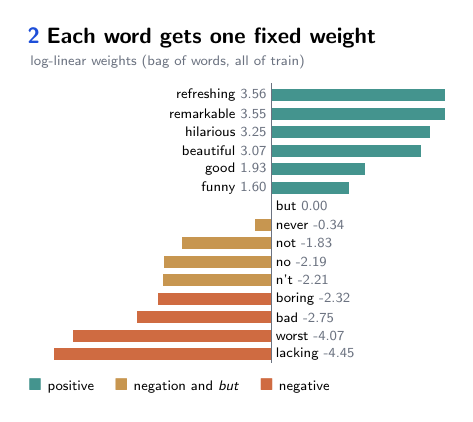
\begin{tikzpicture}[x=1cm,y=1cm]
  \node[ttl] at (0,0.3) {\num{2}Each word gets one fixed weight};
  \node[note,anchor=west] at (0,0.12) {log-linear weights (bag of words, all of train)};
  \def\c{3.1}    % zero line
  \def\k{0.62}   % cm per weight unit
  \foreach \i/\word/\v/\col in {
     0/refreshing/3.56/pos, 1/remarkable/3.55/pos, 2/hilarious/3.25/pos, 3/beautiful/3.07/pos,
     4/good/1.93/pos, 5/funny/1.60/pos,
     6/but/0.00/amber, 7/never/-0.34/amber, 8/not/-1.83/amber, 9/no/-2.19/amber, 10/n't/-2.21/amber,
     11/boring/-2.32/neg, 12/bad/-2.75/neg, 13/worst/-4.07/neg, 14/lacking/-4.45/neg}{
    \pgfmathsetmacro{\y}{-0.3-\i*0.235}
    \fill[\col!78] (\c,{\y+0.075}) rectangle ({\c+\v*\k},{\y-0.075});
    \pgfmathparse{\v>0 ? 1 : 0}
    \ifnum\pgfmathresult=1
      \node[anchor=east,inner sep=1.5pt,font=\tiny] at (\c,\y) {\word\ \lab{\v}};
    \else
      \node[anchor=west,inner sep=1.5pt,font=\tiny] at (\c,\y) {\word\ \lab{\v}};
    \fi}
  \draw[muted] (\c,-0.15) -- (\c,-3.7);
  \node[anchor=west,inner sep=0,font=\tiny] at (0,-4.0) {\textcolor{pos!78}{$\blacksquare$} positive \quad \textcolor{amber!78}{$\blacksquare$} negation and \emph{but} \quad \textcolor{neg!78}{$\blacksquare$} negative};
\end{tikzpicture}
\end{column}
\end{columns}
\end{frame}

\end{document}
